
\begin{frame}[t]
    \frametitle{Содержание теоремы}
    \begin{itemize}
        \item Паросочетание в графе $G$ называется \textcolor{blue}{совершенным}, если оно покрывает все вершины графа $G$.
        \item Обозначим за $odd(G)$ (или  $o(G)$) количество компонент связности графа, содержащих нечётное количество вершин. 
        \item Мы готовы сформулировать теорему. 
    \end{itemize}

    \begin{theorem}[W. T. Tutte, 1947]
       В графе $G$ существует совершенное паросочетание тогда и только тогда, когда для любого $S \subset V(G)$ выполняется условие $odd(G-S) \leq \left| S \right| $.
    \end{theorem}
\end{frame}

\begin{frame}[t]
    \frametitle{Доказательство теоремы}
    \framesubtitle{Туда}
    \renewcommand{\qedsymbol}{}
        \fbox{$ \Rightarrow $} Пусть $M$ -- совершенное паросочетание, $S \subset V(G)$. Тогда граф $G - S$ разобьётся на чётные и нечётные компоненты. Тогда для каждой нечётной компоненты $C$ существует вершина, которая не покрыта рёбрами из $M \cap C$, но \textcolor{blue}{она была покрыта}. Значит, одна вершина из нечётной компоненты связности смежна ребром из паросочетания $M$ с вершиной из множества $S$ (потому что только его мы и удаляли). Все вершины, с которыми соединены вершины из нечётных компонент, разные, потому что из вершины паросочетания выходит ровно 1 ребро. Отсюда следует, что в $S$ вершин не меньше, чем $odd(G-S)$ 
\end{frame}


\begin{frame}[t]
    \frametitle{Доказательство теоремы}
    \framesubtitle{Обратно}
        \fbox{$ \Leftarrow $} \begin{itemize}
            \item Предположим, что граф удовлетворяет условию, но не имеет совершенного паросочетания. Тогда, в частности (подставим $S = \emptyset$), $odd(G) \leq |\emptyset| = 0$, то есть, \textcolor{blue}{$v(G)$ чётно} (потому что в $G$ нет нечётных компонент).
            \item Пусть $G^*$ -- максимальный надграф G на том же множестве вершин, не имеющий совершенного паросочетания (то есть, добавив любое ребро, совершенное паросочетание уже будет). \textcolor{blue}{Мы построим совершенное паросочетание в $G^*$ и придем к противоречию} (фактически главная идея доказательства).
        \end{itemize}
\end{frame}

\begin{frame}[t]
    \begin{itemize}
        \item Пусть $U = \left\{ u \in V(G): d_{G^{*}}(u) = v(G) - 1  \right \}$ (множество вершин, соединённых со всеми остальными). $G^{*}$ -- не полный граф, а значит, $U \neq V(G)$. Удалим эти вершины из $G^*$.

             \begin{figure}[h]
                \centering
                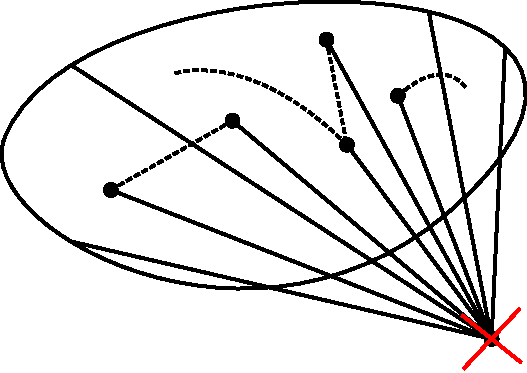
\includegraphics[width=0.5\textwidth]{images/gstar1}
                \label{fig:gstar}
            \end{figure}
        \item (Лемма) Утверждается, что получившийся граф $G^* - U$ -- это \textcolor{blue}{объединение нескольких несвязанных полных графов}. Доказывать будем от противного. 
    \end{itemize}
    
\end{frame}


\begin{frame}[t]
    \frametitle{Доказательство леммы}
    \begin{proof}[Доказательство]
        \renewcommand{\qedsymbol}{}
        \begin{itemize}
            \item Предположим, что это не так. Тогда существуют такие вершины $x, y , z \in  V (G ) \backslash U$, что $xy , yz \in  E (G ^* )$, но $xz \notin  E (G^* )$.
                
            \item Так как $y \notin U$, существует такая вершина $w \notin U$, что $yw \notin E (G^*)$.
            \item Ввиду максимальности графа $G^*$ существует совершенное паросочетание \textcolor{red}{$M_1$ в графе $G^* + xz$} и совершенное паросочетание \textcolor{blue}{$M_2$ в графе $G^* + yw$}. Так как в графе $G^*$ нет совершенного паросочетания, $xz \in M_1$ и $yw \in  M_2$.
                \begin{figure}[h]
                    \centering
                    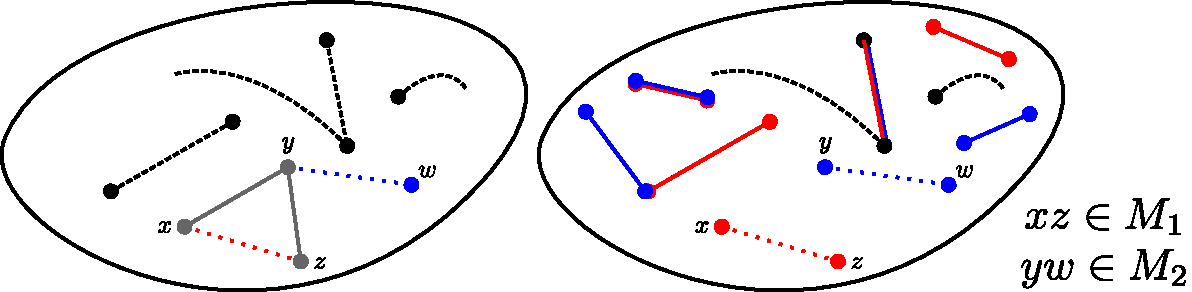
\includegraphics[width=0.8\textwidth]{images/fullgraph2}
                    \label{fig:fullgraph1}
                \end{figure}
        \end{itemize}
    \end{proof}
\end{frame}

\begin{frame}[t]
    \begin{itemize}
        \item Пусть $H = (V (G ), M_1 \triangle M_2 )$. Граф $H$ -- несвязное объединение циклов чётной длины, потому что из каждой вершины  графа $H$ выходит или 0, или 2 ребра (можно вспомнить критерий двудольности графа и применить его для каждой из компонент). Очевидно, в каждом из циклов чередуются рёбра паросочетаний $M_1$ и $M_2$. Из-за чередования рёбер \textcolor{green}{диагоналей} в циклах быть не может. 2 случая: 

            \vspace{5mm}
        \textbf{Случай 1.} $xz$ и $yw$ в разных компонентах $C_1$ и $C_2$ графа $H$

            \begin{figure}[b]
                \centering
                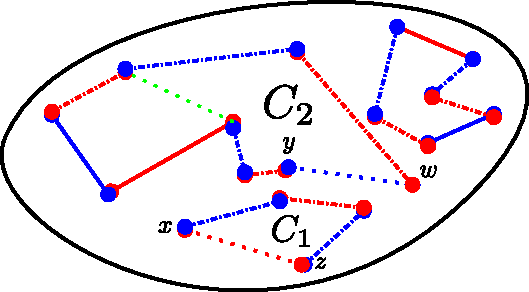
\includegraphics[width=0.5\textwidth]{images/case1}
                \label{fig:case1}
            \end{figure}
    \end{itemize}
\end{frame}

\begin{frame}[t]
                \begin{figure}[h]
                    \centering
                    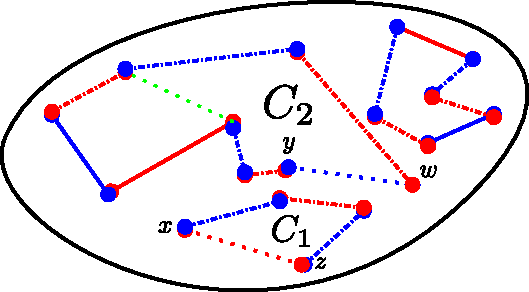
\includegraphics[width=0.4\textwidth]{images/case1}
                    \label{fig:case1}
                \end{figure}

            \begin{itemize}
                \item Тогда на вершинах $C_1$ мы выберем \textcolor{blue}{рёбра паросочетания $M_2$}, на вершинах $C_2$ мы выберем \textcolor{red}{рёбра паросочетания $M_1$ }, а в остальных компонентах графа $H$ -- любое из этих паросочетаний (на рисунке $M_1$).

                \item В итоге получится совершенное паросочетание графа
$G^*$ , противоречие.
                \begin{figure}[h]
                    \centering
                    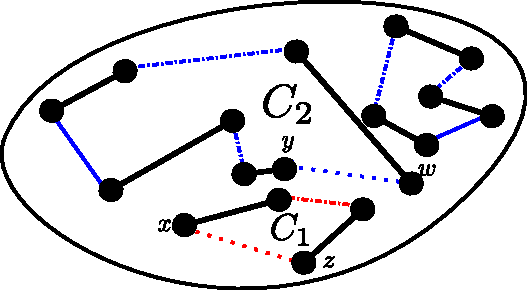
\includegraphics[width=0.4\textwidth]{images/case1_counterproof}
                    \label{fig:case1_counterproof}
                \end{figure}
            \end{itemize}
\end{frame}

\begin{frame}[t]
    \small
    \textbf{Случай 2.} Рёбра $xz$ и $yw$ лежат в одной компоненте $C$ графа $H$.

    \begin{itemize}
        \item В силу симметричности $x$ и $z$ можно считать, что
вершины расположены в чётном цикле $C$ в порядке $ywxz$.
        \item Рассмотрим простой путь $P = zCyxCw$, который состоит из двух дуг цикла  $C$ и ребра $xy$ (оно не в графе $H$, но точно у нас было в $G^*$!). Тогда  $V(P) = V(C)$ и  $E(P) \subset E(G^*)$. Количество рёбер между точками $z, y$ и $x, w$ чётно (иначе рёбра не чередуются). Итак, мы получили путь, убрав ребра $xz, yw$ из чётного цикла и добавив ребро $xy$ $ \Rightarrow $ осталось нечётное количество рёбер. Очевидно, в простом пути нечётной длины существует совершенное паросочетание. \hfill \qedsymbol
    \end{itemize}
    \begin{figure}[h]
        \centering
        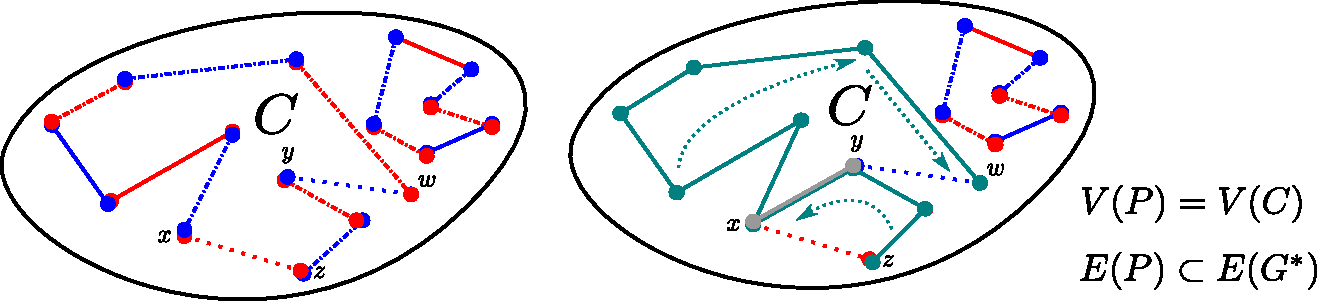
\includegraphics[width=\textwidth]{images/case2_counterproof}
        \label{fig:case2_counterproof}
    \end{figure}
\end{frame}

\begin{frame}[t]
    \frametitle{Доказательство теоремы}
    \begin{itemize}
        \item По лемме $G^* -U$ -- объединение несвязных полных графов. В силу условия, среди них не более чем  $|U|$ имеет нечётное число вершин ($odd(G^* - U) \leq |U|$).
        \item В каждой чётной компоненте графа $G^* - U$ существует совершенное паросочетание, в каждой нечётной -- паросочетание, покрывающее все вершины, кроме одной. Соединим её с вершиной из $U$ (используем различные, и их точно хватит, т. к. $odd(G^* - U) \leq |U|$).
        \item Разбиваем оставшиеся вершины в $U$: они разобьются на пары: это возможно всегда, потому что в изначальном графе (а значит и в $G^*$, потому что $V(G^*) = V(G)$ по построению) количество вершин чётно, а вершины из $U$ -- это \textit{те вершины, которые соединены с остальными по построению}. \hfill \qedsymbol{}
    \end{itemize}
\end{frame}

\begin{frame}[t]
    \frametitle{Рисунок к последним пунктам}
    \framesubtitle{Мы молодцы}
    \begin{figure}[h]
        \centering
        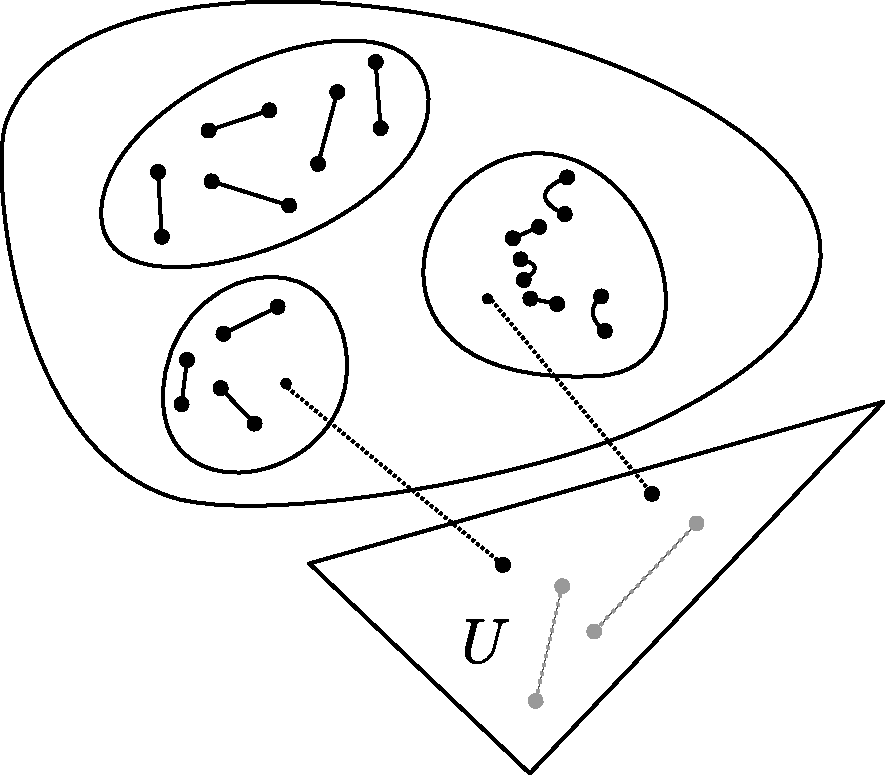
\includegraphics[width=0.8\textwidth]{images/final}
        \label{fig:final}
    \end{figure}
\end{frame}
